\documentclass[tikz, border=10pt]{standalone}
\usepackage{tikz}
\usetikzlibrary{shapes, arrows.meta, positioning, arrows, shadows}

\begin{document}

\tikzstyle{startstop} = [rectangle, rounded corners, minimum width=3cm, minimum height=1cm, text centered, draw=white, fill=red!10]
\tikzstyle{io} = [rectangle, minimum width=3cm, minimum height=1cm, text centered, draw=white, fill=blue!10]
\tikzstyle{process} = [rectangle, minimum width=3cm, minimum height=1cm, text centered, draw=white, fill=orange!10]
\tikzstyle{decision} = [diamond, minimum width=3cm, minimum height=1cm, text centered, draw=white, fill=green!15]
\tikzstyle{arrow} = [thick,->,>=stealth]

\begin{tikzpicture}[node distance=2cm]

% Nodes
\node (start) [startstop] {Research question};
\node (data) [io, below of=start] {Data};
\node (prior) [io, below of=data] {Prior Model};
\node (params) [process, below of=prior] {Parameters};
\node (likelihood) [process, below of=params] {Likelihood};
\node (mcmc) [process, below of=likelihood] {Markov Chain Monte Carlo (MCMC)};
\node (posterior) [process, below of=mcmc] {Posterior Probability};
\node (hdi) [process, below of=posterior] {Highest Density Interval (HDI)};
\node (end) [startstop, below of=hdi] {Review Inferences};

% Arrows
\draw [arrow] (start) -- (data);
\draw [arrow] (data) -- (prior);
\draw [arrow] (prior) -- (params);
\draw [arrow] (params) -- (likelihood);
\draw [arrow] (likelihood) -- (mcmc);
\draw [arrow] (mcmc) -- (posterior);
\draw [arrow] (posterior) -- (hdi);
\draw [arrow] (hdi) -- (end);

\end{tikzpicture}

\begin{figure}
  \centering
  \begin{tikzpicture}[node distance=2cm]

    % Nodes
    \node (data) [process] {Data};
    \node (prior) [process, below=of data] {Prior};
    \node (model) [process, below=of prior] {Model};
    \node (params) [process, below=of model] {Parameters};
    \node (likelihood) [process, below=of params] {Likelihood};
    \node (mcmc) [process, below=of likelihood] {MCMC};
    \node (posterior) [process, below=of mcmc] {Posterior Probability};
    \node (hdi) [process, below=of posterior] {HDI};

    % Arrows
    \draw [arrow] (data) -- (prior);
    \draw [arrow] (prior) -- (model);
    \draw [arrow] (model) -- (params);
    \draw [arrow] (params) -- (likelihood);
    \draw [arrow] (likelihood) -- (mcmc);
    \draw [arrow] (mcmc) -- (posterior);
    \draw [arrow] (posterior) -- (hdi);

  \end{tikzpicture}
  \caption{Standard Bayesian Analysis Flowchart}
\end{figure}


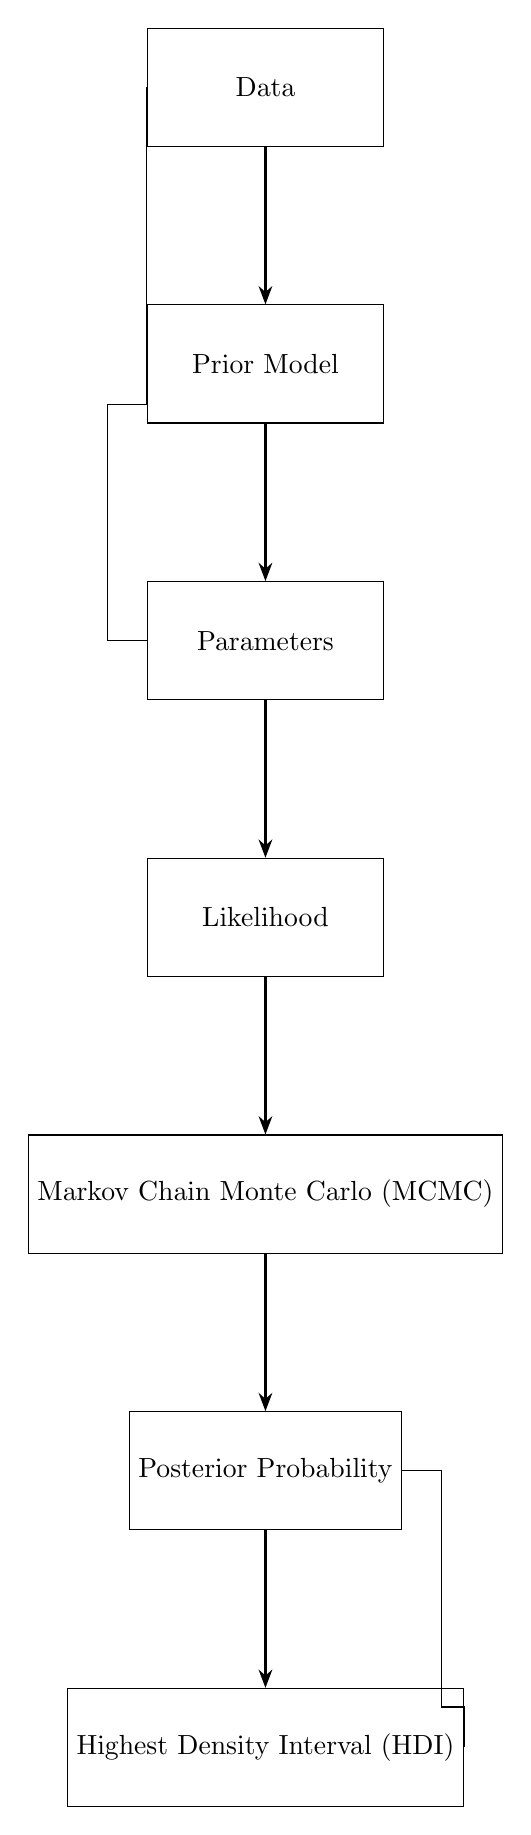
\begin{tikzpicture}[
  node distance=2cm,
  box/.style={
    draw,
    rectangle,
    align=center,
    minimum height=1.5cm,
    minimum width=3cm
  },
  arrow/.style={
    ->,
    >=Stealth,
    thick
  },
  line/.style={
    thin
  }
]

% Nodes
\node[box] (data) {Data};
\node[box, below=of data] (prior) {Prior Model};
\node[box, below=of prior] (params) {Parameters};
\node[box, below=of params] (likelihood) {Likelihood};
\node[box, below=of likelihood] (mcmc) {Markov Chain Monte Carlo (MCMC)};
\node[box, below=of mcmc] (posterior) {Posterior Probability};
\node[box, below=of posterior] (hdi) {Highest Density Interval (HDI)};

% Arrows
\draw[arrow] (data) -- (prior);
\draw[arrow] (prior) -- (params);
\draw[arrow] (params) -- (likelihood);
\draw[arrow] (likelihood) -- (mcmc);
\draw[arrow] (mcmc) -- (posterior);
\draw[arrow] (posterior) -- (hdi);

% Connecting lines
\draw[line] (params.west) -- ++(-0.5,0) -- ++(0,3) -| (data.west);
\draw[line] (posterior.east) -- ++(0.5,0) -- ++(0,-3) -| (hdi.east);

\end{tikzpicture}


\end{document}
